\scanpage{41}
\texttt{/*JOB=CRAY2,ACCT=*********,ALL=M06}\qquad\texttt{J0231CNU}

\texttt{// JOB MSGLEVEL=(0,0),MSGCLASS=Z}

\texttt{// EXEC CSSBATCH}

\texttt{//CRAYIN DD *}

\uline{Oct. 4 83}

\diagram{\begin{tikzcd}[ampersand replacement=\&,column sep=large,row sep=large]
\unsure{\mathbb R}=\unsure{RR}/\sigma_1\arrow[d]\&
\overset{\sigma_0,\sigma_1}{\unsure{RR}}\arrow[l]\arrow[d,"\mathrm{supp}"]\\
A=\vec A/\sigma\&
\vec A\arrow[l]\arrow[loop below,"\sigma"]\&
\vec A_0\arrow[l,leftrightarrow]\arrow[d,"\sigma"]\\
\&\&S\arrow[r,"g"]\&\mathbb N
\end{tikzcd}}

a) $\sigma^2=\mathrm{id}$, $\sigma$ ss pt fixe

b) supp compatible avec $\mathbb D_\infty\longrightarrow\{\pm1\}$

c) $\unsure{RR}/\mathbb D_\infty\underset{\unsure{\exists!}}{\longleftrightarrow}
 A=\vec A/\{\pm1\}$

d) (\unsure{évt}) condition additionnelle (cs hyperboliques) :
$\forall s\in S$, on a
$\deleted{\unsure{2g(s)}}:\ 2g(s)+\nu_s\ge3$
\margin{\[
3\unsure{g_s|g_p}-3+\nu_s\ge0
\]
\[
2\unsure{g_s|g_p}-2+\nu_s\ge1
\]
\[
2g_s+\nu_s\ge3
\]}

1) Somme $+$

\diagram{\(\begin{array}{rl}
4)\ \big\{&\text{amalgamation (\uline{\unsure{sous|sans}} gommage)}\\
5)&\text{découpage (en gardant données de recollement)}\\[1ex]
2)\ \big\{&\text{gommage de \deleted{\unsure{repères}} sommets de marquage.}\\
3)&\text{surmarquage}
\end{array}\)}
\figure{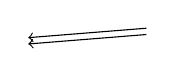
\begin{tikzpicture}
\draw[<-] (0,0)--(1.5,.12);\draw[<-] (0,-.08)--(1.5,.04);
\end{tikzpicture}}
6) Bouchage des trous (gommage des cercles de raccord)

7) \uline{gommage} de cercles de découpage

\margin{4,5 inverses l'un de l'autre (à condition que l'on ne découpe que par
des cercles \uline{marqués})}

\margin{\uline{Cercles de découpage}

\uline{Cercles de raccord}

Sommets de marquage \unsure{ou rigidification|antirigidification}
$\left\{\begin{array}{l}\text{périphériques}\\\text{intérieurs}\end{array}\right.$

Cercles marqués (non marqués)}
\margin{\uline{graphes pondérés}

graphes bipondérés \deleted{\unsure{marqués}}

graphes pondérés marqués}

\uline{Le foncteur twist} $\tau_r$ $(r\in\mathbb Q)$ relatif à un cercle de
découpage marqué, est défini en termes de 4) 5), avec
$\tau_r=\mathrm{id}$ si $r\in\mathbb Z$.
\diagram{\fbox{\begin{tikzcd}[ampersand replacement=\&]
S_1\unsure{\mathcal T}_{g,\nu}^{\pm1}\arrow[r]\&
\unsure{\mathcal T}_{g,\nu}^{\pm1}\arrow[r]\&
\mathrm{Ens}(\unsure{\nu})\times\unsure{[\pm1]|[\mathrm I\mid J]}
\end{tikzcd}}}
\deleted{$\unsure{\mathcal T_{g,\nu}^{\pm}\ \mathcal T_{\mathrm{top}}\
(TSD)_{g,\nu}}$}
\[
\unsure{T_{g,\nu}S_\alpha}
\]

Mais l'\uline{iso} de \uline{twist} \deleted{\unsure{est un}} relatif à
un cercle (de découpage ou de raccord, marqué ou pas),
\inserted{\unsure{ou de recollement}}
$\tau_r$ (pour un cercle de découpage) est une
\uline{nouvelle opération} \unsure{importante}.

\margin{type combinatoire d'un objet de
$\deleted{\unsure{\mathcal T}},\ SD\unsure{\mathcal T}_{\mathrm{top}}$

Catégorie des types combinatoires

\diagram{\(\begin{array}{cc}
\deleted{\mathcal T S}&\deleted{\mathcal T D}\\
\multicolumn{2}{c}{\deleted{\mathcal T SD}}
\end{array}\)}
$\unsure{\text{avec inv}}^{\pm}$
\deleted{$\unsure{\mathcal T^*(\Gamma)}$}

$\unsure{\mathcal T}$

\diagram{\(\begin{array}{c|c}
S\mathcal T&ST\\
SD\mathcal T&SDT\\
D\mathcal T&DT
\end{array}\)}

\diagram{\begin{tikzcd}[ampersand replacement=\&,column sep=small]
\&\mathcal T\arrow[dl,dash]\arrow[dr,dash]\&
\text{graphes pond. discrets}\\
S\mathcal T\arrow[dr,dash]\& \&D\mathcal T\arrow[dl,dash]\\
\&SD\mathcal T\&
\end{tikzcd}}
\unsure{graphes b}\qquad\text{graphes pondérés}\qquad\text{graphes}

\diagram{\begin{tikzcd}[ampersand replacement=\&,column sep=small]
\&t\arrow[dl,dash]\arrow[dr,dash]\&\\
st\arrow[dr,dash]\&\&dt\arrow[dl,dash]\\
\&sdt\&
\end{tikzcd}}}
\mspage{40}
